\scanpage{13}
\diagram{\begin{tikzcd}[ampersand replacement=\&,column sep=2.3em,row sep=2.2em]
1\arrow[r]\&Z\arrow[r,dash]\&G\arrow[r,dash]\&\Gamma\arrow[r,dash]\&1\&[3.2em](E)\\
1\arrow[r,dash]\&Z\arrow[u,"\unsure{2|\wr}"']\arrow[r,dash]\&G'\arrow[u]\arrow[r,dash]
 \&\Gamma'\arrow[u]\arrow[r,dash]\&1\&(E')
\end{tikzcd}}

Si l'extension $(E)$ \unsure{splitte|splitt.}, l'ext. $E'$ aussi.

% Raised abbreviated label and its curved, headless lead to Toute.
\noindent

\begin{tikzpicture}[baseline=(t.base)]
\node[anchor=base west,inner sep=0] (t) at (0,0) {Toute};
\node[anchor=base west,inner sep=0] at (-.12,.63) {\inserted{Rmq}};
\draw[line width=.4pt] (-.15,.14) .. controls (-.20,.43) and (.42,.43) .. (.79,.62);
\end{tikzpicture}
extension splittée $G$ de un $\Gamma$ par un $Z$ provient par image inverse d'\deleted{\unsure{une}}l'ext. splittée
% The formula stands alone at the left; the divider is lower and to its right.
% The two remote marks and the point below the lower rule are not assigned punctuation.
\figure{\begin{tikzpicture}[x=.009cm,y=.009cm]
\node[anchor=base west,inner sep=0] at (0,0) {$\displaystyle Z.\operatorname{Aut}(Z).$};
\node[inner sep=0] at (875,39) {\unsure{\begin{tikzpicture}[x=1pt,y=1pt,baseline=-.3ex]
 \draw[line width=.7pt,line cap=round] (0,1.5)--(.4,.7);
 \fill (.5,-.6) ellipse (.4pt and .6pt);
\end{tikzpicture}}};
\draw[line width=.5pt] (503,-82)--(739,-72);
\draw[line width=.45pt] (511,-102)--(724,-100);
\node[inner sep=0] at (729,-107) {\unsure{\begin{tikzpicture}[baseline=-.3ex]
 \fill (0,0) circle (.25pt);
\end{tikzpicture}}};
\node[inner sep=0] at (1034,-94) {\unsure{\begin{tikzpicture}[baseline=-.3ex]
 \fill (0,0) circle (.3pt);
\end{tikzpicture}}};
\end{tikzpicture}}

4) \quad Ens. de petit cardinal

a) \uline{Cardinal 2}\qquad Ens de cardinal 2 $\longleftrightarrow$ \unsure{torseur|torseurs} \unsure{sur|sous} $\mathbb{Z}_2$ ou encore, \uline{espace affine \unsure{\deleted{sous}|\deleted{sur}|sous|sur}} $\deleted{\unsure{\mathbb{Z}|Z}}\mathbb{F}_2$ (ou encore, \deleted{\illegible{1}} espace affine de dim 1 sur corps $\mathbb{F}_2$ --- car les espaces vect. de dim 1 sur $\mathbb{F}_2$ sont can. isomorphes \ldots)

% Two bent border strokes leave the upper-left and lower-right corners unjoined.
% The parenthetical statement is below the right half of the enclosure.
\figure{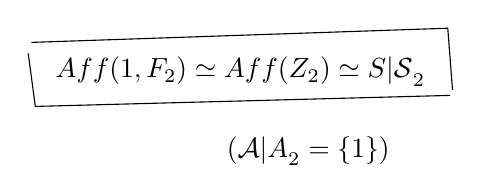
\begin{tikzpicture}
\node[anchor=base west,inner sep=0] (bx) at (0,0)
 {$\displaystyle \operatorname{Aff}(1,\mathbb{F}_2)\simeq
 \operatorname{Aff}(\mathbb{Z}_2)\simeq\unsure{\mathfrak{S}|\mathcal{S}}_2$};
\draw ([xshift=-.30cm,yshift=.18cm]bx.north west)
 -- ([xshift=.28cm,yshift=.36cm]bx.north east)
 -- ([xshift=.34cm,yshift=-.04cm]bx.south east);
\draw ([xshift=-.34cm,yshift=.04cm]bx.north west)
 -- ([xshift=-.25cm,yshift=-.25cm]bx.south west)
 -- ([xshift=.31cm,yshift=-.11cm]bx.south east);
\node[anchor=base east,inner sep=0] at ([xshift=-.45cm,yshift=-.90cm]bx.south east)
 {$\displaystyle (\unsure{\mathcal{A}|A}_2=\{1\})$};
\end{tikzpicture}}

b) \uline{Cardinal 3}
\[
\begin{array}{@{}c@{\;}c@{\;}c@{\;}c@{\;}c@{\;}c@{\;}c@{}}
\mathfrak{S}_3&\simeq&\operatorname{Aff}(1,\mathbb{F}_3)&\simeq&\operatorname{Gl}(2,\mathbb{F}_2)&\simeq&\operatorname{GP}(1,\mathbb{F}_2)\\
&&\rotatebox{90}{$\simeq$}&&&&\rotatebox{90}{$=$}\\
&&\mathbb{F}_3^{+}\mathbin{.}\mathbb{F}_3^{*}&&&&\operatorname{Gl}(2,\mathbb{F}_2)/\mathbb{F}_2^{*}\\[-.3ex]
&&\begin{array}{@{}c@{\qquad}c@{}}\rotatebox{90}{$\unsure{\simeq|=}$}&\rotatebox{90}{$=$}\end{array}&&&&\\[-.3ex]
&&\begin{array}{@{}c@{\qquad}c@{}}\mathbb{Z}_3&\mathbb{Z}_2\end{array}&&&&
\end{array}
\]
\[
\mathcal{A}_3\simeq\deleted{\unsure{\mathbb{Z}|Z}}\mathbb{F}_3^{+}(\simeq\mathbb{Z}_3)
\]
% archive sheet number: 12
